\chapter{Specifikacija programske potpore}
		
	\section{Funkcionalni zahtjevi}		
	
	\noindent \textbf{Dionici:}
	
	\begin{packed_enum}
		
		\item Vlasnik ( naručitelj )
		\item Korisnici
		\begin{packed_enum}
			\item Smještajni administrator 
			\item Administrator prijevoznih usluga 
			\item Korisnički administrator
		\end{packed_enum}			
		\item Razvojni tim 
		
	\end{packed_enum}
	
	\noindent \textbf{Aktori i njihovi funkcionalni zahtjevi:}
	
	
	\begin{packed_enum}
		\item  \underbar{Neprijavljeni korisnik (inicijator) može:}
		
		\begin{packed_enum}
			
			\item se prijaviti u sustav za što su mu potrebni e-mail i lozinka
			
		\end{packed_enum}
		
		\item  \underbar{Smještajni administrator ( inicijator ) može:}
		
		\begin{packed_enum}
			
			\item unositi nove smještaje
			\item mijenjati osnovne podatke smještaja
			\item brisati smještaje
			\item unositi nove korisnike
			\item dodjeljivati uloge korisnicima
			
		\end{packed_enum}
		
		\item  \underbar{Administrator prijevoznih usluga ( inicijator ) može:}
		
		\begin{packed_enum}
			
			\item unositi nove prijevoznike
			\item mijenjati podatke prijevoznika
			\item brisati prijevoznike
			\item unositi vozila za prijevoznike
			\item brisati vozila
			
		\end{packed_enum}
		
		\item  \underbar{Korisnički administrator ( inicijator ) može:}
		
		\begin{packed_enum}
			
			\item unositi pacijente
			
		\end{packed_enum}
		
		\item  \underbar{Baza podataka ( sudionik ) može:}
		
		\begin{packed_enum}
			
			\item pohranjuje sve podatke o korisnicima i njihovim ovlastima 
			\item pohranjuje sve podatke o pacijentu
			\item pohranjuje sve podatke o medicinskoj usluzi 
			\item pohranjuje sve podatke o smještaju 
			\item pohranjuje sve podatke o prijevozniku i vozilima
			\item pohranjuje sve podatke o rezerviranju smještaja 
			\item pohranjuje sve podatke o rezerviranju prijevoznika 
			
		\end{packed_enum}
		
		\item  \underbar{Aplikacija medicinske usluge ( sudionik ):}
		
		\begin{packed_enum}
			
			\item odgovorna za prikupljanje podatak o medicinskim tretmanima te naša aplikacija putem sučelja dohvaća podatke o tretmanima korisnika
			
		\end{packed_enum}
		
		
	\end{packed_enum}
	
	\eject 
			
			
				
			\subsection{Obrasci uporabe}				
					
					\noindent \underbar{\textbf{UC1 - prijava}}
					\begin{packed_item}
	
						\item \textbf{Glavni sudionik:} neprijavljeni  korisnik
						\item  \textbf{Cilj:} dobiti pristup korisničkom sučelju 
						\item  \textbf{Sudionici:} baza podataka
						\item  \textbf{Opis osnovnog tijeka:}
						
						\item[] \begin{packed_enum}
	
							\item Na zahtjev se otvara stranica administratoru
							\item Administrator prenosi podatke korisnika u sustav
							\item Pohranjuju se promjene u bazi podataka
						\end{packed_enum}
						
					\end{packed_item}


                        \noindent \underbar{\textbf{UC2 - odjava}}
					\begin{packed_item}
	
						\item \textbf{Glavni sudionik:} administrator
						\item  \textbf{Cilj:} odjaviti korisnika iz sustava
						\item  \textbf{Sudionici:} baza podataka
                            \item  \textbf{Preduvjet:} korisnik mora postojati u sustavu, odnosno biti već u bazi podataka; administator mora biti prijavljen u sustav
						\item  \textbf{Opis osnovnog tijeka:}
						
						\item[] \begin{packed_enum}
	
							\item Administrator odabire opciju odjave korisnika iz sustava
							\item Korisnik je odjavljen iz sustava i pohranjene su promjene
       
						\end{packed_enum}
						
					\end{packed_item}

                        \noindent \underbar{\textbf{UC3 - pregled svih administratora}}
					\begin{packed_item}
	
						\item \textbf{Glavni sudionik:} smještajni administrator
						\item  \textbf{Cilj:} dobiti uvid u podatke svih administratora
						\item  \textbf{Sudionici:} baza podataka
						\item  \textbf{Preduvjet:} administrator je prijavljen i dodijeljena mu je uloga smještajnog administratora
						\item  \textbf{Opis osnovnog tijeka:}
						
						\item[] \begin{packed_enum}
	
							\item Smještajni administrator odabire opciju pregleda svih administratora kojima je on nadležan - korisničkih administratora i administratora prijevoznih usluga
							\item Otvara se popis svih administratora 
							
						\end{packed_enum}
						
					\end{packed_item}

                        \noindent \underbar{\textbf{UC4 - unos novog administratora}}
					\begin{packed_item}
	
						\item \textbf{Glavni sudionik: }smještajni administrator
						\item  \textbf{Cilj:} dodati administratora
						\item  \textbf{Sudionici:} baza podataka
						\item  \textbf{Preduvjet:} administrator je prijavljen i dodijeljena mu je uloga smještajnog administratora
						\item  \textbf{Opis osnovnog tijeka:}
						
						\item[] \begin{packed_enum}
	
							\item Smještajni administrator odabere opciju dodavanja novog administratora
							\item Otvara se prozor za unos podataka
							\item Smještajni administrator upiše podatke o novom administratoru
							\item U bazu podataka se pohrani promjena
							
						\end{packed_enum}
						
						\item  \textbf{Opis mogućih odstupanja:}
						
						\item[] \begin{packed_item}
	
							\item[3.a] Upisano je neispravno korisničko ime administratora
							\item[] \begin{packed_enum}
								
								\item Sustav obavještava smještajnog administratora o neuspjelom upisu
								
							\end{packed_enum}
					
						\end{packed_item}
					\end{packed_item}

                        \noindent \underbar{\textbf{UC5 - brisanje administratora}}
					\begin{packed_item}
	
						\item \textbf{Glavni sudionik: }smještajni administrator
						\item  \textbf{Cilj:} obrisati administratora
						\item  \textbf{Sudionici:} baza podataka
						\item  \textbf{Preduvjet:} administrator je prijavljen i dodijeljena mu je uloga smještajnog administratora
						\item  \textbf{Opis osnovnog tijeka:}
						
						\item[] \begin{packed_enum}
	
							\item Smještajni administrator odabere opciju brisanja administratora
							\item Otvara se prozor za unos podataka
							\item Smještajni administrator upiše podatke o administratoru
							\item Smještajni administrator odabere opciju 'Izbriši'
							\item Administrator se uklanja iz baze podataka
						\end{packed_enum}
					
					\end{packed_item}

                        \noindent \underbar{\textbf{UC6 - dodjeljivanje uloga}}
					\begin{packed_item}
	
						\item \textbf{Glavni sudionik: } smještajni administrator
						\item  \textbf{Cilj:} dodijeliti ulogu administratoru
						\item  \textbf{Sudionici:} baza podataka
						\item  \textbf{Preduvjet:} administrator je prijavljen i dodijeljena mu je uloga smještajnog administratora
						\item  \textbf{Opis osnovnog tijeka:}
						
						\item[] \begin{packed_enum}
	
							\item Smještajni administrator otvara popis svih administratora
							\item Smještajni administrator odabere administratora kojem želi promijeniti ulogu
							\item Otvori se prozor s podatcima administratora
							\item Smještajni administrator odabere jednu od ponuđenih uloga (korisnički administrator ili administrator prijevoznih usluga)
							\item U bazu podataka se pohrani promjena
						\end{packed_enum}
						
						\item  \textbf{Opis mogućih odstupanja:}
						
						\item[] \begin{packed_item}
	
							\item[3.a] Upisano je neispravno korisničko ime administratora
							\item[] \begin{packed_enum}
								
								\item Sustav obavještava smještajnog administratora o neuspjelom dodjeljivanju uloge administratoru
								
							\end{packed_enum}
			
						\end{packed_item}
					\end{packed_item}

                        \noindent \underbar{\textbf{UC7 - pregled svih smještaja}}
					\begin{packed_item}
	
						\item \textbf{Glavni sudionik: }smještajni administrator
						\item  \textbf{Cilj:} pregledati sve smještaje
						\item  \textbf{Sudionici:} baza podataka
						\item  \textbf{Preduvjet:} administrator je prijavljen i dodijeljena mu je uloga smještajnog administratora, postoji barem jedan smještaj unesen u sustav
						\item  \textbf{Opis osnovnog tijeka:}
						
						\item[] \begin{packed_enum}
	
							\item Administrator odabere opciju pregleda svih smještaja
							\item Prikaže se popis svih smještaja koji postoje u sustavu
							
						\end{packed_enum}
						
					\end{packed_item}

                        \noindent \underbar{\textbf{UC8 - pregled smještaja}}
					\begin{packed_item}
	
						\item \textbf{Glavni sudionik: }smještajni administrator
						\item  \textbf{Cilj:} pregledati traženi smještaj
						\item  \textbf{Sudionici:} baza podataka
						\item  \textbf{Preduvjet:} administrator je prijavljen i dodijeljena mu je uloga smještajnog administratora
						\item  \textbf{Opis osnovnog tijeka:}
						
						\item[] \begin{packed_enum}
	
							\item Administrator odabere opciju pregleda svih smještaja
							\item Prikaže se popis svih smještaja koji postoje u sustavu
							\item Administrator odabere iz popisa traženi smještaj
						
						\end{packed_enum}
						
					\end{packed_item}

                        \noindent \underbar{\textbf{UC9 - unos novog smještaja}}
					\begin{packed_item}
	
						\item \textbf{Glavni sudionik: }smještajni administrator
						\item  \textbf{Cilj:} dodati novi smještaj
						\item  \textbf{Sudionici:} baza podataka
						\item  \textbf{Preduvjet:} administrator je prijavljen i dodijeljena mu je uloga smještajnog administratora
						\item  \textbf{Opis osnovnog tijeka:}
						
						\item[] \begin{packed_enum}
	
							\item Administrator odabere opciju dodavanja smještaja
							\item Otvara se prozor za unos podataka o novom smještaju
							\item Administrator unese podatke o smještaju
							\item U bazu podataka se pohrani promjena
						\end{packed_enum}
						
						\item  \textbf{Opis mogućih odstupanja:}
						
						\item[] \begin{packed_item}
	
							\item[3.a] Upisano je neispravno ime smještaja
							\item[] \begin{packed_enum}
								
								\item Sustav obavještava smještajnog administratora o neuspjelom upisu
								
							\end{packed_enum}
       
						\end{packed_item}
					\end{packed_item}

                        \noindent \underbar{\textbf{UC10 - izmjena podataka o smještaju}}
					\begin{packed_item}
	
						\item \textbf{Glavni sudionik: }smještajni administrator
						\item  \textbf{Cilj:} izmijeniti podatke o smještaju
						\item  \textbf{Sudionici:} baza podataka
						\item  \textbf{Preduvjet:} administrator je prijavljen i dodijeljena mu je uloga smještajnog administratora
						\item  \textbf{Opis osnovnog tijeka:}
						
						\item[] \begin{packed_enum}
	
							\item Administrator odabere opciju pregleda svih smještaja
							\item Prikaže se popis svih smještaja koji postoje u sustavu
							\item Administrator odabere iz popisa traženi smještaj 
							\item Otvori se stranica s podatcima o smještaju
							\item Administrator izmijeni podatke o smještaju
                                \item Administrator odabere opciju 'Spremi promjene'
                                \item U bazu podataka se pohrani promjena
						\end{packed_enum}
						
						\item  \textbf{Opis mogućih odstupanja:}
						
						\item[] \begin{packed_item}
	
							\item[3.a] Traženi smještaj ne postoji u sustavu
							\item[] \begin{packed_enum}
								
								\item Sustav obavještava smještajnog administratora da smještaj ne postoji u sustavu
								
							\end{packed_enum}
							
						\end{packed_item}
					\end{packed_item}

                        \noindent \underbar{\textbf{UC11 - brisanje smještaja}}
					\begin{packed_item}
	
						\item \textbf{Glavni sudionik: }smještajni administrator
						\item  \textbf{Cilj:} obrisati smještaj
						\item  \textbf{Sudionici:} baza podataka
						\item  \textbf{Preduvjet:} administrator je prijavljen i dodijeljena mu je uloga smještajnog administratora
						\item  \textbf{Opis osnovnog tijeka:}
						
						\item[] \begin{packed_enum}
	
							\item Administrator odabere opciju brisanja smještaja
							\item Otvara se prozor za unos podataka
							\item Administrator unese ime smještaja i obriše ga
							\item Smještaj se uklanja iz baze podataka
						\end{packed_enum}
						
						
					\end{packed_item}


                        \noindent \underbar{\textbf{UC12 - prikaz smještaja na karti}}
					\begin{packed_item}
	
						\item \textbf{Glavni sudionik: }smještajni administrator
						\item  \textbf{Cilj:} prikazati smještaj na karti
						\item  \textbf{Sudionici:} OpenMaps
						\item  \textbf{Preduvjet:} administrator je prijavljen i dodijeljena mu je uloga smještajnog administratora
						\item  \textbf{Opis osnovnog tijeka:}
						
						\item[] \begin{packed_enum}
	
							\item Administrator odabire opciju pregleda svih smještaja
							\item Prikaže se popis svih smještaja koji postoje u sustavu
							\item Administrator odabere iz popisa traženi smještaj
							\item Administrator odabere opciju prikaza smještaja na karti
							\item Otvori se prozor gdje se vidi lokacija smještaja na karti
						\end{packed_enum}
						
						\item  \textbf{Opis mogućih odstupanja:}
						
						\item[] \begin{packed_item}
	
							\item[3.a] Traženi smještaj ne postoji u sustavu
							\item[] \begin{packed_enum}
								
								\item Sustav obavještava smještajnog administratora da smještaj ne postoji u sustavu
								
							\end{packed_enum}
							\item[4.a] Smještaj se ne može locirati na karti
							\item[] \begin{packed_enum}
								
								\item Sustav obavještava smještajnog administratora da smještaj nije moguće locirati
								
							\end{packed_enum}
							
						\end{packed_item}
					\end{packed_item}


                        \noindent \underbar{\textbf{UC13 - pregled prijevoznika}}
					\begin{packed_item}
	
						\item \textbf{Glavni sudionik: }administrator prijevoznih usluga
						\item  \textbf{Cilj:} pregledati sve prijevoznike
						\item  \textbf{Sudionici:} baza podataka
						\item  \textbf{Preduvjet:} administrator je prijavljen i dodijeljena mu je uloga administratora prijevoznih usluga; postoji barem jedan prijevoznik u sustavu
						\item  \textbf{Opis osnovnog tijeka:}
						
						\item[] \begin{packed_enum}
	
							\item Administrator odabere opciju pregleda svih prijevoznika
							\item Prikaže se popis svih prijevoznika
							\item Administrator odabere traženog prijevoznika
       
						\end{packed_enum}
						
					\end{packed_item}


                        \noindent \underbar{\textbf{UC14 - izmjena podataka prijevoznika}}
					\begin{packed_item}
	
						\item \textbf{Glavni sudionik: }administrator prijevoznih usluga
						\item  \textbf{Cilj:} izmijeniti podatke traženog administratora
						\item  \textbf{Sudionici:} baza podataka
						\item  \textbf{Preduvjet:} administrator je prijavljen i dodijeljena mu je uloga administratora prijevoznih usluga; postoji barem jedan prijevoznik u sustavu
						\item  \textbf{Opis osnovnog tijeka:}
						
						\item[] \begin{packed_enum}
	
							\item Administrator odabire opciju pregleda svih prijevoznika
                                \item Prikaže se popis svih prijevoznika koji postoje u sustavu
                                \item Administrator odabere iz popisa traženog prijevoznika
                                \item Otvori se stranica s podatcima prijevoznika
                                \item Administrator izmijeni podatke o prijevozniku
                                \item Administrator odabere opciju 'Spremi promjene'
                                \item U bazu podataka se pohrani promjena
						\end{packed_enum}
						
						\item  \textbf{Opis mogućih odstupanja:}
						
						\item[] \begin{packed_item}
	
							\item[3.a] Traženi prijevoznik ne postoji u sustavu
							\item[] \begin{packed_enum}
								
								\item Sustav obavještava administratora da odabrani prijevoznik ne postoji u sustavu
								
							\end{packed_enum}
			
						\end{packed_item}
					\end{packed_item}

                        \noindent \underbar{\textbf{UC15 - unos novog vozila}}
					\begin{packed_item}
	
						\item \textbf{Glavni sudionik: }administrator prijevoznih usluga
						\item  \textbf{Cilj:} unijeti podatke o novom vozilu
						\item  \textbf{Sudionici:} baza podataka
						\item  \textbf{Preduvjet:} administrator je prijavljen i dodijeljena mu je uloga administratora prijevoznih usluga
						\item  \textbf{Opis osnovnog tijeka:}
						
						\item[] \begin{packed_enum}
	
							\item Administrator odabere opciju dodavanja novog vozila
							\item Otvara se prozor za unos podataka o novom vozilu
							\item Administrator unese podatke o vozilu
							\item U bazu podataka se pohrani promjena
						\end{packed_enum}
						
						
					\end{packed_item}

                        \noindent \underbar{\textbf{UC16 - brisanje vozila}}
					\begin{packed_item}
	
						\item \textbf{Glavni sudionik: }administrator prijevoznih usluga
						\item  \textbf{Cilj:} obrisati vozilo
						\item  \textbf{Sudionici:} baza podataka
						\item  \textbf{Preduvjet:} administrator je prijavljen i dodijeljena mu je uloga administratora prijevoznih usluga
						\item  \textbf{Opis osnovnog tijeka:}
						
						\item[] \begin{packed_enum}
	
							\item Administrator odabere opciju brisanja vozila
							\item Otvara se prozor za unos podataka
							\item Administrator unese ime vozila i obriše ga
							\item Vozilo se uklanja iz baze podataka
						\end{packed_enum}
						
						
					\end{packed_item}

                        \noindent \underbar{\textbf{UC17 - pregled svih prijevoznika}}
					\begin{packed_item}
	
						\item \textbf{Glavni sudionik: }administrator prijevoznih usluga
						\item  \textbf{Cilj:} dobiti uvid u sve prijevoznike
						\item  \textbf{Sudionici:} baza podataka
						\item  \textbf{Preduvjet:} administrator je prijavljen i dodijeljena mu je uloga administratora prijevoznih usluga
						\item  \textbf{Opis osnovnog tijeka:}
						
						\item[] \begin{packed_enum}
	
							\item Administrator odabire opciju pregleda svih prijevoznika
							\item Prikaže se popis svih prijevoznika
							
						\end{packed_enum}
						
					\end{packed_item}


                        \noindent \underbar{\textbf{UC18 - brisanje prijevoznika}}
					\begin{packed_item}
	
						\item \textbf{Glavni sudionik: }administrator prijevoznih usluga
						\item  \textbf{Cilj:} obrisati prijevoznika
						\item  \textbf{Sudionici:} baza podataka
						\item  \textbf{Preduvjet:} administrator je prijavljen i dodijeljena mu je uloga administratora prijevoznih usluga
						\item  \textbf{Opis osnovnog tijeka:}
						
						\item[] \begin{packed_enum}
	
							\item Administrator odabire opciju brisanja prijevoznika
							\item Otvara se prozor za unos podataka
                                \item Administrator unese ime prijevoznika i obriše ga
                                \item Prijevoznik se uklanja iz baze podataka
						\end{packed_enum}
						
					\end{packed_item}

                        \noindent \underbar{\textbf{UC19 - unos novog prijevoznika}}
					\begin{packed_item}
	
						\item \textbf{Glavni sudionik: }administrator prijevoznih usluga
						\item  \textbf{Cilj:} unijeti novog prijevoznika
						\item  \textbf{Sudionici:} baza podataka
						\item  \textbf{Preduvjet:} administrator je prijavljen i dodijeljena mu je uloga administratora prijevoznih usluga
						\item  \textbf{Opis osnovnog tijeka:}
						
						\item[] \begin{packed_enum}
	
							\item Administrator odabire opciju dodavanja prijevoznika
                                \item Otvara se prozor za unos podataka o novom prijevozniku
                                \item Administrator unese podatke o prijevozniku
                                \item Administrator odabere opciju 'Dodaj prijevoznika'
                                \item U bazu podataka se pohrani promjena
						\end{packed_enum}
						
						\item  \textbf{Opis mogućih odstupanja:}
						
						\item[] \begin{packed_item}
	
							\item[3.a] Upisano je neispravno ime prijevoznika
							\item[] \begin{packed_enum}
								
								\item Sustav obavještava administratora o neuspjelom unosu
								
							\end{packed_enum}
							
						\end{packed_item}
					\end{packed_item}

                        \noindent \underbar{\textbf{UC20 - unos novog pacijenta}}
					\begin{packed_item}
	
						\item \textbf{Glavni sudionik: }korisnički administrator
						\item  \textbf{Cilj:} unijeti podatke o novom pacijentu
						\item  \textbf{Sudionici:} baza podataka, aplikacija medicinskih usluga
						\item  \textbf{Preduvjet:} administrator je prijavljen u sustav i ima ulogu korisničkog administratora
						\item  \textbf{Opis osnovnog tijeka:}
						
						\item[] \begin{packed_enum}
	
							\item Administrator odabire opciju unosa novog pacijenta
                                \item Otvara se prozor za upis podataka novog pacijenta
                                \item Administrator upiše podatke o novom pacijentu
                                \item Pohranjuju se promjene u bazu podataka
						\end{packed_enum}
						
					\end{packed_item}

                        \noindent \underbar{\textbf{UC21 - dohvaćanje termina pacijenta}}
					\begin{packed_item}
	
						\item \textbf{Glavni sudionik: }korisnički administrator
						\item  \textbf{Cilj:} dohvatiti podatke o terminu medicinskih usluga
						\item  \textbf{Sudionici:} baza podataka, aplikacij medicinskih usluga
						\item  \textbf{Preduvjet:} administrator je prijavljen u sustav i ima ulogu korisničkog administratora
						\item  \textbf{Opis osnovnog tijeka:}
						
						\item[] \begin{packed_enum}

                                \item Administrator otvara aplikaciju medicinskih usluga
							\item Administrator iz aplikacije medicinskih usluga preuzima podatke preferiranog dolaska i odlaska pacijenta
                                \item Podatci o terminu se upisuju u sustav
                                \item Pohranjuju se promjene u bazu podataka
						\end{packed_enum}
						
						\item  \textbf{Opis mogućih odstupanja:}
						
						\item[] \begin{packed_item}
	
							\item[2.a] Za navedeno razdoblje dolaska i odlaska nema dostupnih termina
							\item[] \begin{packed_enum}
								
								\item Sustav javlja administratoru da u navedenom razdoblju nema dostupnih termina
								
							\end{packed_enum}
							
						\end{packed_item}
					\end{packed_item}

                        \noindent \underbar{\textbf{UC22 - dodjeljivanje smještaja pacijentu}}
					\begin{packed_item}
	
						\item \textbf{Glavni sudionik: }korisnički administrator
						\item  \textbf{Cilj:} +dodijeliti smještaj pacijentu
						\item  \textbf{Sudionici:} baza podataka, aplikacija medicinskih usluga
						\item  \textbf{Preduvjet:} administrator je prijavljen u sustav i ima ulogu korisničkog administratora
						\item  \textbf{Opis osnovnog tijeka:}
						
						\item[] \begin{packed_enum}
	
							\item Smještajni administrator unosi u aplikaciju podatke o raspoloživom smještaju
                                \item Administrator unosi korisnika u sustav
                                \item Administrator pridjeljuje raspoloživu smještajnu jedinicu
                                \item Smještajna jedinica se označava kao zauzeta u danom periodu
						\end{packed_enum}
						
					\end{packed_item}

                       

                        \noindent \underbar{\textbf{UC23 - dodjeljivanje prijevoznika terminima}}
					\begin{packed_item}
	
						\item \textbf{Glavni sudionik: }korisnički administrator
						\item  \textbf{Cilj:} dodijeliti prijevoznika
						\item  \textbf{Sudionici:} baza podataka, aplikacija medicinskih usluga
						\item  \textbf{Preduvjet:} administrator je prijavljen u sustav i ima ulogu korisničkog administratora 
						\item  \textbf{Opis osnovnog tijeka:}
						
						\item[] \begin{packed_enum}
	
							\item Administrator prijevoznih usluga u aplikaciju unosi podatke o prijevoznicima
                                \item Administrator unosi korisnika u sustav
                                \item Zaključavanje plana medicinskih usluga s listom termina
                                \item Administrator pridjeljuje raspoložive prijevoznike za svaki od termina
                                \item Administrator označava prijevoznike zauzete u tim terminima
						\end{packed_enum}
						
					\end{packed_item}

     				

     			\noindent \underbar{\textbf{UC24 - slanje e-maila prijevozniku}}
					\begin{packed_item}
	
						\item \textbf{Glavni sudionik: }korisnički administrator
						\item  \textbf{Cilj:} poslati e-mail s podatcima korisnika prijevozniku
						\item  \textbf{Sudionici:} baza podataka, aplikacija medicinskih usluga
						\item  \textbf{Preduvjet:} administrator je prijavljen u sustav i ima ulogu korisničkog administratora 
						\item  \textbf{Opis osnovnog tijeka:}
						
						\item[] \begin{packed_enum}
	
							\item Plan o medicinskim uslugama je zaključan
       				\item Aplikacija dohvaća e-mail adresu prijevoznika
       				\item Aplikacija unutar predloška za e-mail postavlja podatke o medicinskoj uslugi i pojedinostima 
	   			\item Na e-mail adresu prijevoznika se šalje plan 
						\end{packed_enum}

      						\item  \textbf{Opis mogućih odstupanja:}
						
						\item[] \begin{packed_item}
	
							\item[3.a] Podatci u aplikaciji ne kooperiraju sa podatcima prijevoznika
							\item[] \begin{packed_enum}
								
								\item Sustav upozorava da je došlo do pogrešne korelacije podataka
								
							\end{packed_enum}
							
						\end{packed_item}
						
					\end{packed_item}


     			\noindent \underbar{\textbf{UC25 - slanje e-maila pacijentu}}
					\begin{packed_item}
	
						\item \textbf{Glavni sudionik: }korisnički administrator
						\item  \textbf{Cilj:} poslati e-mail s pojedinostima termina pacijentu
						\item  \textbf{Sudionici:} baza podataka, aplikacija medicinskih usluga
						\item  \textbf{Preduvjet:} administrator je prijavljen u sustav i ima ulogu korisničkog administratora 
						\item  \textbf{Opis osnovnog tijeka:}
						
						\item[] \begin{packed_enum}
	
							\item Plan o medicinskim uslugama je zaključan
       				\item Dohvaća se e-mail adresa pacijenta
       				\item Aplikacija unutar e-maila postavlja pojedinosti o terminu medicinske usluge - termin, prijevoznika, smještaj
	   			\item Na e-mail adresu pacijenta se šalje plan
						\end{packed_enum}

      						\item  \textbf{Opis mogućih odstupanja:}
						
						\item[] \begin{packed_item}
	
							\item[3.a] Podatci u aplikaciji ne kooperiraju sa pacijentovim podatcima
							\item[] \begin{packed_enum}
								
								\item Sustav upozorava da je došlo do pogrešne korelacije podataka
								
							\end{packed_enum}
							
						\end{packed_item}
						
					\end{packed_item}
                        
				
					
				\subsubsection{Dijagrami obrazaca uporabe}
					
					\begin{figure}[H]
						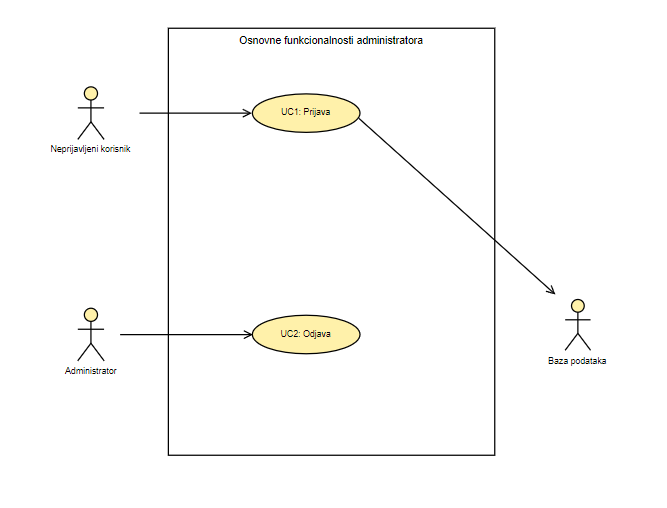
\includegraphics[width=\textwidth]{slike/uc1.PNG} %veličina u odnosu na širinu linije
						\caption{Dijagram obrasca uporabe, osnovne funkcionalnosti administratora}
						\label{fig:uc1} %label mora biti drugaciji za svaku sliku
					\end{figure}
					
					\begin{figure}[H]
						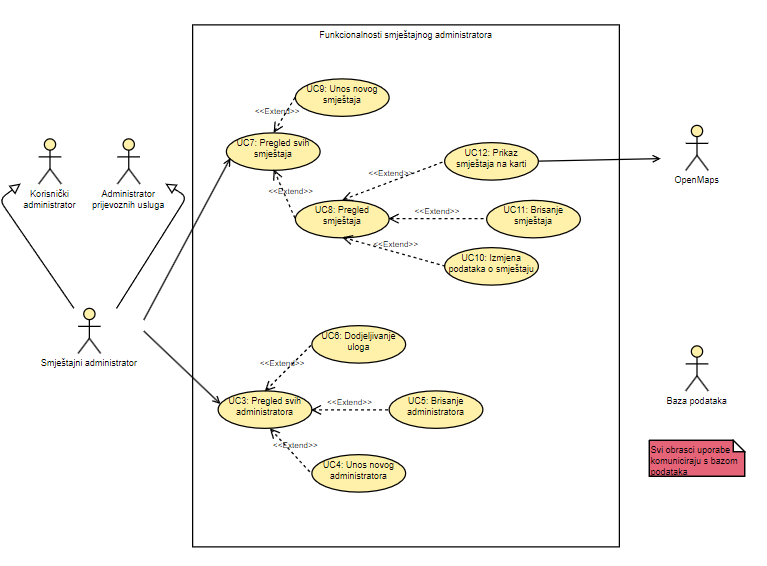
\includegraphics[width=\textwidth]{slike/uc2.PNG} %veličina u odnosu na širinu linije
						\caption{Dijagram obrasca uporabe, funkcionalnosti smještajnog administratora}
						\label{fig:uc2} %label mora biti drugaciji za svaku sliku
					\end{figure}
					
					\begin{figure}[H]
						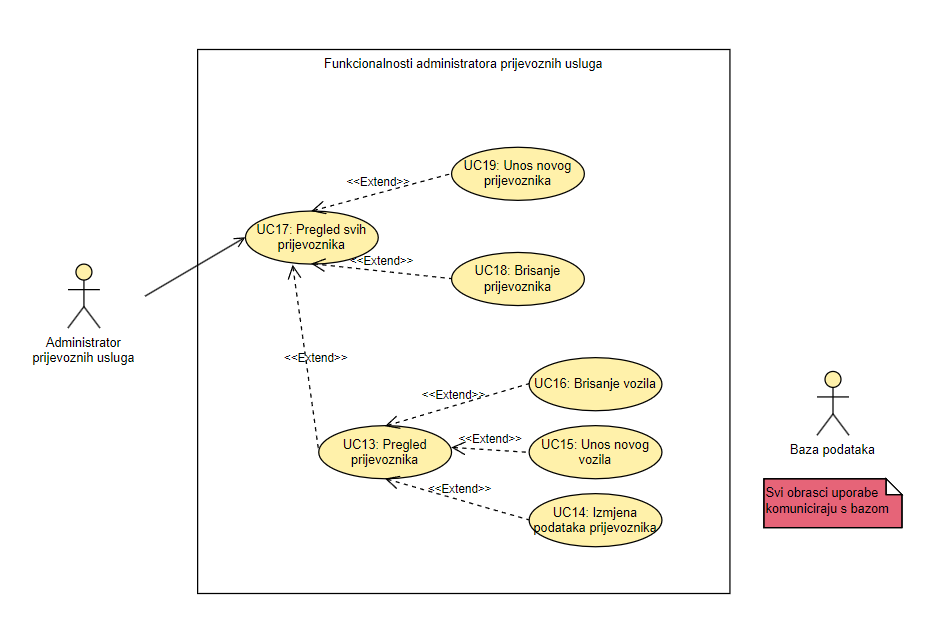
\includegraphics[width=\textwidth]{slike/uc3.PNG} %veličina u odnosu na širinu linije
						\caption{Dijagram obrasca uporabe, funkcionalnosti administratora prijevoznih usluga} 
						\label{fig:uc3} %label mora biti drugaciji za svaku sliku
					\end{figure}
					
					\begin{figure}[H]
						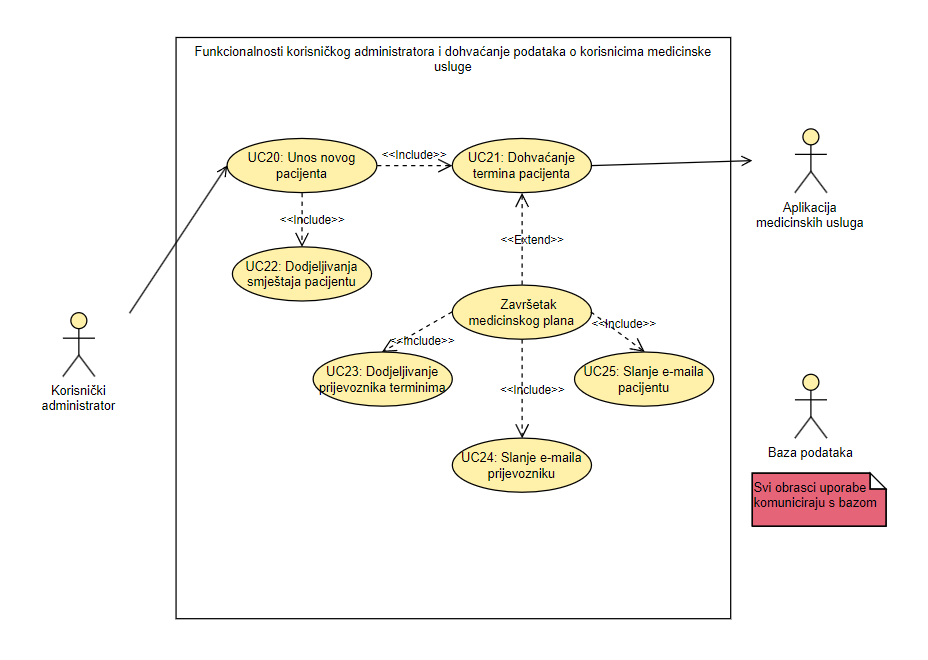
\includegraphics[width=\textwidth]{slike/uc4.PNG} %veličina u odnosu na širinu linije
						\caption{Dijagram obrasca uporabe, funkcionalnosti korisničkog administratora}
						\label{fig:uc4} %label mora biti drugaciji za svaku sliku
					\end{figure}
					
				\eject		
				
			\subsection{Sekvencijski dijagrami}
			
				\paragraph{Prijava – obrazac uporabe UC1}\mbox{} \\
				\noindent Neregistrirani korisnik odabire gumb “Prijavi se” te ga se preusmjeruje na stranicu s formom za prijavu. Ovdje upisuje svoj e-mail i lozinku te klikom na gumb ”Nastavi” uneseni podaci se šalju na validaciju. Ukoliko se podaci podudaraju s onima pohranjenima  u bazi, dostavljaju se informacije o administratoru te token za određene uloge koje administrator ima. Ovisno o tokenu, administratoru postaje dostupno korisničko sučelje prilagođeno njegovoj ulozi ili ulogama. U suprotnom, ako uneseni podaci ne odgovaraju niti jednom administratoru u bazi, korisnik prima obavijest o pogreški kako bi znao da nije registriran u sustavu. 
				
				\begin{figure}[H]
					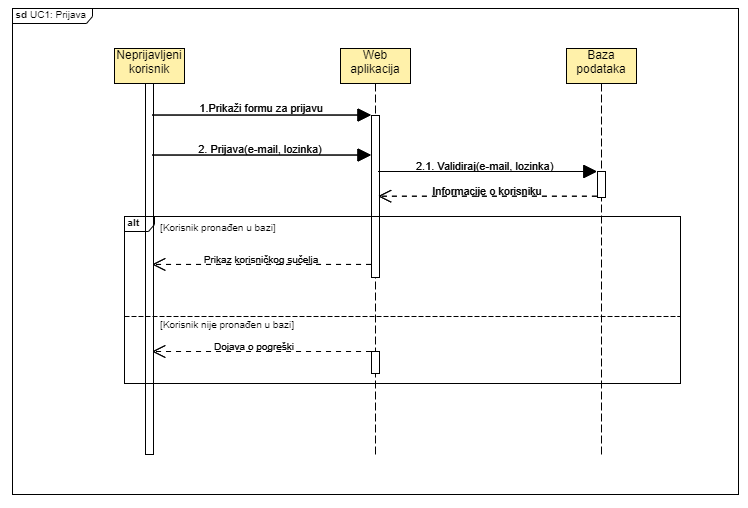
\includegraphics[width=\textwidth]{slike/sd1.PNG} %veličina u odnosu na širinu linije
					\caption{Sekvencijski dijagram za UC1}
					\label{fig:sd1} %label mora biti drugaciji za svaku sliku
				\end{figure}
				
				
				\eject
	
		\section{Ostali zahtjevi}
		
			\begin{packed_item}
				\setlength\itemsep{10pt}
				\item Aplikacija mora osigurati visoku razinu pouzdanosti u evidenciji i koordinaciji smještaja i prijevoza, uz minimalnu grešku u podacima.
				\item Sučelje treba biti intuitivno i prilagođeno korisnicima koji možda nisu upoznati s aplikacijama sličnog sadržaja.
				\item Vrijeme odziva aplikacije na korisničke zahtjeve treba biti brzo kako bi se osiguralo učinkovito upravljanje rezervacijama.
				\item Aplikacija treba podržavati veliki broj korisnika i smještajnih kapaciteta, uz mogućnost lakoće nadogradnje za dodatne kapacitete.
				\item Sigurnosni protokoli za zaštitu osobnih podataka korisnika i osjetljivih informacija o rezervacijama su neophodni.
				\item Aplikacija treba biti kompatibilna s postojećim sustavima za administraciju zdravstvenih usluga.
				\item Aplikacija treba osigurati efikasno upravljanje uslugama kako bi se zadovoljile potrebe i očekivanja klijenata.
				\item Aplikacija mora omogućiti efikasno praćenje i upravljanje rezervacijama smještaja i prijevoza, s detaljnim izvještajima o statusu i dostupnosti.
				\item Aplikacija treba biti dizajnirana s fokusom na efikasnost i jednostavnost navigacije, omogućujući brzu i laku upotrebu bez nepotrebnih vizualnih distrakcija.
			\end{packed_item}
			 
			 
			 
	
